\documentclass{ximera}

%\usepackage{todonotes}

\newcommand{\todo}{}

\usepackage{esint} % for \oiint
\ifxake%%https://math.meta.stackexchange.com/questions/9973/how-do-you-render-a-closed-surface-double-integral
\renewcommand{\oiint}{{\large\bigcirc}\kern-1.56em\iint}
\fi


\graphicspath{
  {./}
  {ximeraTutorial/}
  {basicPhilosophy/}
  {functionsOfSeveralVariables/}
  {normalVectors/}
  {lagrangeMultipliers/}
  {vectorFields/}
  {greensTheorem/}
  {shapeOfThingsToCome/}
  {dotProducts/}
  {../productAndQuotientRules/exercises/}
  {../normalVectors/exercisesParametricPlots/}
  {../continuityOfFunctionsOfSeveralVariables/exercises/}
  {../partialDerivatives/exercises/}
  {../chainRuleForFunctionsOfSeveralVariables/exercises/}
  {../commonCoordinates/exercisesCylindricalCoordinates/}
  {../commonCoordinates/exercisesSphericalCoordinates/}
  {../greensTheorem/exercisesCurlAndLineIntegrals/}
  {../greensTheorem/exercisesDivergenceAndLineIntegrals/}
  {../shapeOfThingsToCome/exercisesDivergenceTheorem/}
  {../greensTheorem/}
  {../shapeOfThingsToCome/}
}

\newcommand{\mooculus}{\textsf{\textbf{MOOC}\textnormal{\textsf{ULUS}}}}

\usepackage{tkz-euclide}\usepackage{tikz}
\usepackage{tikz-cd}
\usetikzlibrary{arrows}
\tikzset{>=stealth,commutative diagrams/.cd,
  arrow style=tikz,diagrams={>=stealth}} %% cool arrow head
\tikzset{shorten <>/.style={ shorten >=#1, shorten <=#1 } } %% allows shorter vectors

\usetikzlibrary{backgrounds} %% for boxes around graphs
\usetikzlibrary{shapes,positioning}  %% Clouds and stars
\usetikzlibrary{matrix} %% for matrix
\usepgfplotslibrary{polar} %% for polar plots
\usepgfplotslibrary{fillbetween} %% to shade area between curves in TikZ
\usetkzobj{all}
%\usepackage[makeroom]{cancel} %% for strike outs
%\usepackage{mathtools} %% for pretty underbrace % Breaks Ximera
%\usepackage{multicol}
\usepackage{pgffor} %% required for integral for loops



%% http://tex.stackexchange.com/questions/66490/drawing-a-tikz-arc-specifying-the-center
%% Draws beach ball
\tikzset{pics/carc/.style args={#1:#2:#3}{code={\draw[pic actions] (#1:#3) arc(#1:#2:#3);}}}



\usepackage{array}
\setlength{\extrarowheight}{+.1cm}   
\newdimen\digitwidth
\settowidth\digitwidth{9}
\def\divrule#1#2{
\noalign{\moveright#1\digitwidth
\vbox{\hrule width#2\digitwidth}}}





\newcommand{\RR}{\mathbb R}
\newcommand{\R}{\mathbb R}
\newcommand{\N}{\mathbb N}
\newcommand{\Z}{\mathbb Z}

\newcommand{\sagemath}{\textsf{SageMath}}


%\renewcommand{\d}{\,d\!}
\renewcommand{\d}{\mathop{}\!d}
\newcommand{\dd}[2][]{\frac{\d #1}{\d #2}}
\newcommand{\pp}[2][]{\frac{\partial #1}{\partial #2}}
\renewcommand{\l}{\ell}
\newcommand{\ddx}{\frac{d}{\d x}}

\newcommand{\zeroOverZero}{\ensuremath{\boldsymbol{\tfrac{0}{0}}}}
\newcommand{\inftyOverInfty}{\ensuremath{\boldsymbol{\tfrac{\infty}{\infty}}}}
\newcommand{\zeroOverInfty}{\ensuremath{\boldsymbol{\tfrac{0}{\infty}}}}
\newcommand{\zeroTimesInfty}{\ensuremath{\small\boldsymbol{0\cdot \infty}}}
\newcommand{\inftyMinusInfty}{\ensuremath{\small\boldsymbol{\infty - \infty}}}
\newcommand{\oneToInfty}{\ensuremath{\boldsymbol{1^\infty}}}
\newcommand{\zeroToZero}{\ensuremath{\boldsymbol{0^0}}}
\newcommand{\inftyToZero}{\ensuremath{\boldsymbol{\infty^0}}}



\newcommand{\numOverZero}{\ensuremath{\boldsymbol{\tfrac{\#}{0}}}}
\newcommand{\dfn}{\textbf}
%\newcommand{\unit}{\,\mathrm}
\newcommand{\unit}{\mathop{}\!\mathrm}
\newcommand{\eval}[1]{\bigg[ #1 \bigg]}
\newcommand{\seq}[1]{\left( #1 \right)}
\renewcommand{\epsilon}{\varepsilon}
\renewcommand{\phi}{\varphi}


\renewcommand{\iff}{\Leftrightarrow}

\DeclareMathOperator{\arccot}{arccot}
\DeclareMathOperator{\arcsec}{arcsec}
\DeclareMathOperator{\arccsc}{arccsc}
\DeclareMathOperator{\si}{Si}
\DeclareMathOperator{\scal}{scal}
\DeclareMathOperator{\sign}{sign}


%% \newcommand{\tightoverset}[2]{% for arrow vec
%%   \mathop{#2}\limits^{\vbox to -.5ex{\kern-0.75ex\hbox{$#1$}\vss}}}
\newcommand{\arrowvec}[1]{{\overset{\rightharpoonup}{#1}}}
%\renewcommand{\vec}[1]{\arrowvec{\mathbf{#1}}}
\renewcommand{\vec}[1]{{\overset{\boldsymbol{\rightharpoonup}}{\mathbf{#1}}}}
\DeclareMathOperator{\proj}{\vec{proj}}
\newcommand{\veci}{{\boldsymbol{\hat{\imath}}}}
\newcommand{\vecj}{{\boldsymbol{\hat{\jmath}}}}
\newcommand{\veck}{{\boldsymbol{\hat{k}}}}
\newcommand{\vecl}{\vec{\boldsymbol{\l}}}
\newcommand{\uvec}[1]{\mathbf{\hat{#1}}}
\newcommand{\utan}{\mathbf{\hat{t}}}
\newcommand{\unormal}{\mathbf{\hat{n}}}
\newcommand{\ubinormal}{\mathbf{\hat{b}}}

\newcommand{\dotp}{\bullet}
\newcommand{\cross}{\boldsymbol\times}
\newcommand{\grad}{\boldsymbol\nabla}
\newcommand{\divergence}{\grad\dotp}
\newcommand{\curl}{\grad\cross}
%\DeclareMathOperator{\divergence}{divergence}
%\DeclareMathOperator{\curl}[1]{\grad\cross #1}
\newcommand{\lto}{\mathop{\longrightarrow\,}\limits}

\renewcommand{\bar}{\overline}

\colorlet{textColor}{black} 
\colorlet{background}{white}
\colorlet{penColor}{blue!50!black} % Color of a curve in a plot
\colorlet{penColor2}{red!50!black}% Color of a curve in a plot
\colorlet{penColor3}{red!50!blue} % Color of a curve in a plot
\colorlet{penColor4}{green!50!black} % Color of a curve in a plot
\colorlet{penColor5}{orange!80!black} % Color of a curve in a plot
\colorlet{penColor6}{yellow!70!black} % Color of a curve in a plot
\colorlet{fill1}{penColor!20} % Color of fill in a plot
\colorlet{fill2}{penColor2!20} % Color of fill in a plot
\colorlet{fillp}{fill1} % Color of positive area
\colorlet{filln}{penColor2!20} % Color of negative area
\colorlet{fill3}{penColor3!20} % Fill
\colorlet{fill4}{penColor4!20} % Fill
\colorlet{fill5}{penColor5!20} % Fill
\colorlet{gridColor}{gray!50} % Color of grid in a plot

\newcommand{\surfaceColor}{violet}
\newcommand{\surfaceColorTwo}{redyellow}
\newcommand{\sliceColor}{greenyellow}




\pgfmathdeclarefunction{gauss}{2}{% gives gaussian
  \pgfmathparse{1/(#2*sqrt(2*pi))*exp(-((x-#1)^2)/(2*#2^2))}%
}


%%%%%%%%%%%%%
%% Vectors
%%%%%%%%%%%%%

%% Simple horiz vectors
\renewcommand{\vector}[1]{\left\langle #1\right\rangle}


%% %% Complex Horiz Vectors with angle brackets
%% \makeatletter
%% \renewcommand{\vector}[2][ , ]{\left\langle%
%%   \def\nextitem{\def\nextitem{#1}}%
%%   \@for \el:=#2\do{\nextitem\el}\right\rangle%
%% }
%% \makeatother

%% %% Vertical Vectors
%% \def\vector#1{\begin{bmatrix}\vecListA#1,,\end{bmatrix}}
%% \def\vecListA#1,{\if,#1,\else #1\cr \expandafter \vecListA \fi}

%%%%%%%%%%%%%
%% End of vectors
%%%%%%%%%%%%%

%\newcommand{\fullwidth}{}
%\newcommand{\normalwidth}{}



%% makes a snazzy t-chart for evaluating functions
%\newenvironment{tchart}{\rowcolors{2}{}{background!90!textColor}\array}{\endarray}

%%This is to help with formatting on future title pages.
\newenvironment{sectionOutcomes}{}{} 



%% Flowchart stuff
%\tikzstyle{startstop} = [rectangle, rounded corners, minimum width=3cm, minimum height=1cm,text centered, draw=black]
%\tikzstyle{question} = [rectangle, minimum width=3cm, minimum height=1cm, text centered, draw=black]
%\tikzstyle{decision} = [trapezium, trapezium left angle=70, trapezium right angle=110, minimum width=3cm, minimum height=1cm, text centered, draw=black]
%\tikzstyle{question} = [rectangle, rounded corners, minimum width=3cm, minimum height=1cm,text centered, draw=black]
%\tikzstyle{process} = [rectangle, minimum width=3cm, minimum height=1cm, text centered, draw=black]
%\tikzstyle{decision} = [trapezium, trapezium left angle=70, trapezium right angle=110, minimum width=3cm, minimum height=1cm, text centered, draw=black]

\author{Bart Snapp and Jim Talamo}


\outcome{Define orthogonal decomposition.}
\outcome{Define orthogonal and scalar projections.}
\outcome{Use the dot product in applied settings.}

\title[Dig-In:]{Projections and orthogonal decomposition}

\begin{document}
\begin{abstract}
 Projections tell us how much of one vector lies in the direction of another and are important in physical applications.
\end{abstract}
\maketitle


\section{Projections and components}

\subsection{Projections}
One of the major uses of the dot product is to let us \textit{project}
one vector in the direction of another. Conceptually, we are looking
at the ``shadow'' of one vector projected onto another, sort of like
in the case of a sundial.
\begin{image}%%https://commons.wikimedia.org/wiki/File:Perceton_sundial_-_detail.JPG
  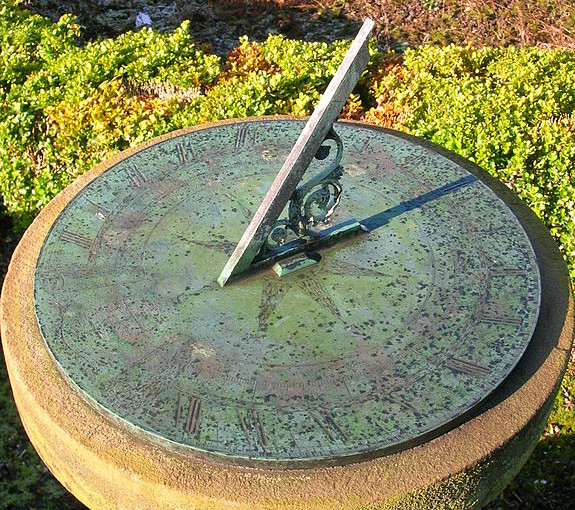
\includegraphics{sundial.jpg}
\end{image}
In essence we imagine the ``sun'' directly over a vector, casting a shadow onto another vector.
\begin{image}
  \begin{tikzpicture}
    \foreach \angle in { 270,280,...,450 }{
      \draw [ultra thick, yellow!70!orange, rotate around={\angle:(3,4)}]
      (3,3.5)--(3,3);
    };
    \draw[very thick, penColor,->] (0,0) -- (5,0);
    \draw[ultra thick,penColor4,->] (0,0) -- (3,2);
    \draw[ultra thick,penColor2,->] (0,0) -- (3,0);
    \draw[ultra thick, yellow!50!orange] (2.5,4)
    arc (180:360:.5);

    \draw[decoration={brace,mirror,raise=.2cm},decorate,thin] (0,0)--(3,0);
    \node at (1.5,-.5) {projection};

  \end{tikzpicture}
\end{image}

While this is good starting point for understanding orthogonal
projections, now we need the definition.

\begin{definition}
  The \dfn{orthogonal projection}\index{projection} of vector $\vec{v}$ in the direction
  of vector $\vec{w}$ is a new vector denoted
  $\proj_\vec{w}(\vec{v})$
  \begin{image}
    \begin{tikzpicture}
      \draw[dashed] (-.5,-.5) -- (3.5,3.5);
      \draw[ultra thick,penColor4,->] (0,0) -- (3,1);
      \draw[ultra thick,penColor2,->] (-0,0) -- (0.707,0.707);
      %\draw[textColor, dashed] (3,1) -- (2,2);
      \node[below] at (1.5, 0.5) [penColor4] {$\vec{v}$};
      \node at (0.2, .5) [penColor2] {$\vec{w}$};
    \end{tikzpicture}
    \qquad
    \begin{tikzpicture}
      \draw[textColor, dashed] (3,1) -- (2,2);
      \draw[textColor, thin] (2.2,1.8) -- (2,1.6)--(1.8,1.8);
      \draw[draw=none] (-.5,-.5) -- (3.5,3.5);
      \draw[very thick, penColor,->] (0,0) -- (2,2);
      \draw[ultra thick,penColor4,->] (0,0) -- (3,1);
      \draw[ultra thick,penColor2,->] (-0,0) -- (0.707,0.707);
      %\node[above] at (1.5, 0.5) [penColor] {$\vec{v}$};
      %\node at (0.2, .5) [penColor2] {$\vec{w}$};
      \node[above left] at (1, 1) [penColor] {$\proj_\vec{w}(\vec{v})$};
    \end{tikzpicture}
  \end{image}
  that lies on the line containing $\vec{w}$, with the vector
  $\proj_\vec{w}(\vec{v}) - \vec{v}$ perpendicular to $\vec{w}$.
  \begin{onlineOnly}
    Below we see vectors $\vec{v}$ and $\vec{w}$ along with
    $\proj_{\vec{w}}(\vec{v})$. Move the tips of vectors $\vec{v}$ and
    $\vec{w}$ to help you understand $\proj_{\vec{w}}(\vec{v})$.
    \begin{center}
      \geogebra{f8bqsRAz}{800}{600}
    \end{center}
\end{onlineOnly}
\end{definition}

\begin{question}
  Consider the vector $\vec{v}=\vector{3,2,1}$ and the vector $\veci =
  \vector{1,0,0}$.  Compute $\proj_\veci(\vec{v})$.
  \begin{hint}
    Draw a picture.
  \end{hint}
  \begin{prompt}
    \[
    \proj_\veci(\vec{v}) = \vector{\answer{3},\answer{0},\answer{0}}
    \]
  \end{prompt}
  \begin{question}
    Let $\vec{v} = \vector{1,1}$ and $\vec{w}=\vector{-1,1}$. Compute
    $\proj_\vec{w}(\vec{v})$.
    \begin{hint}
      Draw a picture.
    \end{hint}
      \begin{prompt}
        \[
        \proj_\vec{w}(\vec{v}) = \vector{\answer{0},\answer{0}}
        \]
      \end{prompt}
  \end{question}
\end{question}

To compute the projection of one vector along another, we use the dot
product.

\begin{theorem}
  Given two vectors $\vec{v}$ and $\vec{w}$
  \[
  \proj_\vec{w}(\vec{v})
  =\left(\frac{\vec{v} \dotp \vec{w}}{|\vec{w}|^2}\right) \vec{w}
  =\left(\frac{\vec{v} \dotp \vec{w}}{\vec{w}\dotp \vec{w}}\right) \vec{w}.
  \]
  \begin{explanation}
    First, note that the direction of $\proj_\vec{w}(\vec{v})$ is given by
    \[
    \frac{\vec{w}}{|\vec{w}|}
    \]
    and the magnitude of $\proj_\vec{w}(\vec{v})$ is given by
    \[
    |\proj_{\vec{w}}(\vec{v})| = |\vec{v}|\cdot \left| \answer[given]{\cos(\theta)}\right|.
    \]
    \begin{image}
      \begin{tikzpicture}
        \draw (.5,.1) arc[radius=.5cm,start angle=11.3,end angle=56.3];
        \draw[->,ultra thick,penColor] (0,0) -- (5,1);
        \draw[->,ultra thick,penColor2] (0,0) -- (2,3);
        \draw[thin] (2.46,.71)--(2.25,.67)--(2.29,0.46);
        \draw[dashed] (2,3) -- (2.5,.5);
        \node[below,penColor] at (3.75,.75) {$\vec{w}$}; %% <a,b>
        \node[above left,penColor2] at (1,1.5) {$\vec{v}$}; %% <c,d>
        \node[above right] at (.4,.2) {$\theta$}; %% <c,d>
        \draw[decoration={brace,mirror,raise=.2cm},decorate,thin] (0,0)--(2.5,.5);
        \node at (1.25,-.25) {$\cos(\theta)$};
      \end{tikzpicture}
    \end{image}
    Now
    \[
    \proj_\vec{w}(\vec{v}) = \mathrm{direction}\cdot\mathrm{magnitude},
    \]
    where
    \[
    \mathrm{direction} = \pm \frac{\vec{w}}{|\vec{w}|}
    \]
    has a positive sign if $0<\theta< \pi/2$, and a negative sign if
    $\pi/2< \theta< \pi$. Also,
    \[
    \mathrm{magnitude} = |\vec{v}|\cdot\left|\answer[given]{\cos(\theta)}\right|.
    \]
    Multiplying direction and magnitude we find the following.
    \begin{align*}
      &= \frac{\vec{w}}{|\vec{w}|^2}\cdot |\vec{w}|\cdot |\vec{v}|\cdot\answer[given]{\cos(\theta)}\\
      &= \left(\frac{\vec{v} \dotp \vec{w}}{|\vec{w}|^2}\right) \vec{w}\\
      &=\left(\frac{\vec{v} \dotp \vec{w}}{\vec{w}\dotp \vec{w}}\right) \vec{w}.
    \end{align*}
    Notice that the sign of the direction is the sign of cosine, so we simply remove the absolute value from the cosine.
  \end{explanation}
\end{theorem}

\begin{question}
  Find the projection of the vector $\vec{v} = \vector{2,3,1}$ in the
  direction of the vector $\vec{w} = \vector{3,-1,1}$.
  \begin{prompt}
  \[
  \proj_\vec{w}(\vec{v}) = \vector{\answer{\frac{12}{11}},\answer{\frac{-4}{11}},\answer{\frac{4}{11}}}
  \]
  \end{prompt}
\end{question}

\begin{question}
  Let $\vec{v}$ and $\vec{w}$ be nonzero vectors in $\R^2$. Let $k\ge
  1$. Select all statements that must be true.
  \begin{selectAll}
    \choice{$\proj_{\vec{w}}(\vec{v})=\proj_{\vec{v}}(\vec{w})$}
    \choice[correct]{$|\proj_{\vec{w}}(\vec{v})|\le |\vec{v}|$}
    \choice{$|\proj_{\vec{w}}(\vec{v})|\le |\vec{w}|$}
    \choice[correct]{$|\proj_{\vec{w}}(\vec{v})|\le |\proj_{\vec{w}}(k\cdot \vec{v})|$}
    \choice{$|\proj_{\vec{w}}(k\cdot \vec{v})|\le |\proj_{\vec{w}}(\vec{v})|$}
    \choice[correct]{$|\proj_{\vec{w}}(\vec{v})|\le |\proj_{k\cdot \vec{w}}(\vec{v})|$}
    \choice[correct]{$|\proj_{k\cdot \vec{w}}(\vec{v})|\le |\proj_{\vec{w}}(\vec{v})|$}
  \end{selectAll}
\end{question}


\subsection{Components}
Scalar components compute ``how much'' of a vector is pointing in a
particular direction.
\begin{definition}
  Let $\vec{v}$ and $\vec{w}$ be vectors and let $0\le\theta\le\pi$ be
  the angle between them.  The \dfn{scalar component}\index{component}
  in the direction of $\vec{w}$ of vector $\vec{v}$ is denoted
  \[
  \scal_\vec{w}(\vec{v})=
  \begin{cases}
    |\proj_\vec{w}(\vec{v})| &\text{when $0\le\theta\le \pi/2$}\\
    -|\proj_\vec{w}(\vec{v})| &\text{when $\pi/2<\theta\le \pi$.}
  \end{cases}
  \]
\end{definition}

\begin{question}
  Let $\vec{v} = \vector{3,-2,1}$. Compute $\scal_\veci(\vec{v})$.
  \begin{prompt}
    \[
    \scal_\veci(\vec{v}) = \answer{3}
    \]
  \end{prompt}
  \begin{question}
    Compute $\scal_\vecj(\vec{v})$.
    \begin{prompt}
      \[
      \scal_\vecj(\vec{v}) = \answer{-2}
      \]
    \end{prompt}
    \begin{question}
      Compute $\scal_\veck(\vec{v})$.
      \begin{prompt}
        \[
        \scal_\veck(\vec{v}) = \answer{1}
        \]
      \end{prompt}
    \end{question}
  \end{question}
\end{question}
To compute the scalar component of a vector in the direction of
another, you use the dot product.

\begin{theorem}
  Given two vectors, $\vec{v}$ and $\vec{w}$,
  \[
  \scal_\vec{w}(\vec{v}) =\frac{\vec{v} \dotp \vec{w}}{|\vec{w}|}.
  \]
\end{theorem}

\begin{question}
  Let $\vec{v}$ and $\vec{w}$ be nonzero vectors and let $\theta$ be
  the angle between them. Which of the following are true?
  \begin{selectAll}
    \choice{$|\proj_\vec{w}(\vec{v})| = \scal_{\vec{w}}(\vec{v})$}
    \choice[correct]{$|\proj_\vec{w}(\vec{v})| = |\scal_{\vec{w}}(\vec{v})|$}
    \choice[correct]{$\proj_\vec{w}(\vec{v}) =|\vec{v}|\cos(\theta)\left(\frac{\vec{w}}{|\vec{w}|}\right)$}
    \choice[correct]{$\scal_\vec{w}(\vec{v}) = |\vec{v}|\cos(\theta)$}
  \end{selectAll}
\end{question}


%%%%%%%%%%
%\section{Orthogonal decomposition}
%In many applications, we need to know how much of one vector lies in the direction of another.  Imagine the following scenarios.
%
%\begin{model}
%A table lies flat on the ground, and a person places a marble on the table and releases it.  Does the marble move? \wordChoice{\choice{Yes.}\choice[correct]{No.}}
%
%Now, the table is tilted, and the person places the marble near the middle of the table and releases it. Does the marble move? \wordChoice{\choice[correct]{Yes.}\choice{No.}}
%
%While this may not seem earth-shattering (unless the marble is really, \emph{really} massive), another interesting observation can be made.  If the marble is placed on the middle of the tilted table and is released, it rolls down the table.  
%
%\begin{question}
%Based off of your physical intuition, how will the speed of the marble depend on the steepness of the table?  If the table is tilted steeply, the marble will roll 
%\wordChoice{\choice[correct]{ faster}\choice{slower}} than it would if the table is tilted less steeply. 
%\end{question}
%
%Physics gives us a way to model this scenario, so we present the argument here, then extract its mathematical essence.  We begin by drawing a ``free body diagram'' in three scenarios - a flat table, a gently steep table, and a steep table.  To draw this, we indicate the forces acting on the marble.  In all cases, the gravitational force $\vec{F_g}$ points directly towards the floor, and a ``normal force'' $\vec{F_n}$ points perpendicular to the table (we note that there must be such a force keeping the marble on the table).  Thus, the normal force perfectly counteracts the part $\vec{F_g}$ that is perpendicular to the table (or the marble would fall through the table).  We thus can resolve the gravitational force into a component perpendicular to the table, denoted by $\vec{F_g}_{, \perp}$ and one parallel to the table, denoted by $\vec{F_g}_{, \parallel}$.
%
% \begin{image}
%    \begin{tikzpicture}
%        \begin{axis}[ymax=1.5,xmax=3.9, ymin=-.8, xmin=-1.9,
%            unit vector ratio*=1 1 1,
%            axis lines=none
%          ]
%                 \addplot[very thick,penColor] plot coordinates {(0,0)(0,.5)(2,.5)(2,0)};
%                	\addplot[color=penColor4,fill=penColor4,only marks,mark=*] coordinates{(1,.57)};
%          \addplot[very thick,penColor5,->] plot coordinates {(1,.5) (1,-.2)};
%          \addplot[very thick,penColor2,->] plot coordinates {(1,.57) (1,1.27)};
%          \node[above] at (axis cs:1.3, .6) [penColor2] {$\vec{F_n}$};
%                    \node[above] at (axis cs:1.3, -.15) [penColor5] {$\vec{F_g}$};
%
%         \node at (axis cs:1, -.5) [black] {\footnotesize The forces are balanced so the marble doesn't move.};
%                      \addplot[very thin,penColor] plot coordinates {(0,-1)};
%        \end{axis}
%    \end{tikzpicture}
%  \end{image}
%
% \begin{image}
%    \begin{tikzpicture}
%        \begin{axis}[ymax=2.5,xmax=3.9, ymin=-.8, xmin=-1.9,
%            unit vector ratio*=1 1 1,
%            axis lines=none
%          ]
%                 \addplot[very thick,penColor] plot coordinates {(0,0)(-.3,.4)(1.6,1.2)(1.9,.8)};
%                	\addplot[color=penColor4,fill=penColor4,only marks,mark=*] coordinates{(.65,.88)};
%          \addplot[very thick,penColor2,->] plot coordinates {(.65,.9) (.25,1.6)};
%          \addplot[very thick,penColor5,->] plot coordinates {(.65,.86) (.65,0)};
%          \node[above] at (axis cs:.95, 1.1) [penColor2] {$\vec{F_n}$};
%                    \node[above] at (axis cs:.25, -.15) [penColor5] {$\vec{F_g}$};
%
%         \node at (axis cs:1, -.5) [black] {\footnotesize The table is tilted gently.};
%                      \addplot[very thin,penColor] plot coordinates {(0,-1)};
%        \end{axis}
%    \end{tikzpicture}
%  \end{image}
%
%
% \begin{image}
%    \begin{tikzpicture}
%        \begin{axis}[ymax=2.5,xmax=3.9, ymin=-.8, xmin=-1.9,
%            unit vector ratio*=1 1 1,
%            axis lines=none
%          ]
%                 \addplot[very thick,penColor] plot coordinates {(0,0)(-.35,.35)(.96,1.76)(1.31,1.41)};
%                	\addplot[color=penColor,fill=penColor,only marks,mark=*] coordinates{(1.13,1.05)};
%          \addplot[very thick,penColor5,->] plot coordinates {(1,.5) (1,0)};
%          \addplot[very thick,penColor2,->] plot coordinates {(1,.5) (1,1)};
%          \node[above] at (axis cs:1.3, .6) [penColor2] {$\vec{F_n}$};
%                    \node[above] at (axis cs:1.3, -.15) [penColor5] {$\vec{F_g}$};
%
%         \node at (axis cs:1, -.5) [black] {\footnotesize The table is tilted steeply.};
%                      \addplot[very thin,penColor] plot coordinates {(0,-1)};
%        \end{axis}
%    \end{tikzpicture}
%  \end{image}
%  
%  Note that in the last two pictures, we use the geometric interpretation of vector addition to draw the components of gravity perpendicular and parallel to the table.
%\end{model}
%




\subsection{Orthogonal decomposition}


Given any vector $\vec{v}$ in $\R^2$, we can always write it as
\[
\vec{v} = a\veci + b\vecj
\]
for some real numbers $a$ and $b$.  Here we've broken $\vec{v}$ into
the sum of two orthogonal vectors --- in particular, vectors parallel to
$\veci$ and $\vecj$. In fact, given a vector $\vec{v}$ and another
vector $\vec{w}$ you can always break $\vec{v}$ into a sum of two
vectors, one of which is parallel to $\vec{w}$ and another that is
perpendicular to $\vec{w}$. Such a sum is called an \textit{orthogonal
  decomposition}.
\begin{onlineOnly}
  Move the point around to see various orthogonal decompositions of
  vector $\vec{v}$.
  \begin{center}
    \geogebra{juszKc6k}{800}{600}
  \end{center}
\end{onlineOnly}

\begin{definition}
Let $\vec v$ and $\vec w$ be vectors. The \dfn{orthogonal
  decomposition} of $\vec v$ in terms of $\vec{w}$ is the sum
\[
\vec v = \underbrace{\proj_{\vec{w}}(\vec{v})}_{\parallel \vec w} +  (\underbrace{\vec v-\proj_{\vec{w}}(\vec{v})}_{\perp \vec w}),
\]
where $\vec{x} \parallel \vec{y}$ means that ``$\vec{x}$ is parallel
to $\vec{y}$'' and $\vec{x} \perp\vec{y}$ means that ``$\vec{x}$ is
perpendicular to $\vec{y}$''.
\end{definition}

\begin{question}
Let $\vec u = \vector{-2,1}$ and $\vec v = \vector{3,1}$.  What is the
orthogonal decomposition of $\vec{u}$ in terms of $\vec{v}$?
\begin{prompt}
\[
\vec u= \underbrace{\vector{\answer{-1.5},\answer{-0.5}}}_{\parallel \vec v} + \underbrace{\vector{\answer{-0.5},\answer{1.5}}}_{\perp \vec v}
\]
\end{prompt}
\begin{question}
  Let $\vec w =\vector{2,1,3}$ and $\vec x  =\vector{ 1,1,1}$. What is the
  orthogonal decomposition of $\vec{w}$ in terms of $\vec{x}$?
  \begin{prompt}
  \[
  \vec w  = \underbrace{\vector{\answer{2},\answer{2},\answer{2}}}_{\parallel \vec x} + \underbrace{\vector{ \answer{0},\answer{-1},\answer{1}}}_{\perp\vec x}
  \]
  \end{prompt}
\end{question}
\end{question}


We conclude this section with a physical example where orthogonal decomposition is useful.

\begin{example}
  Consider a box weighing $50\unit{lb}$ placed on a frictionless ramp that rises
  $5\unit{ft}$ over a span of $20\unit{ft}$.
  \begin{image}
    \begin{tikzpicture}
      \begin{scope}[scale=.25]
	\draw [thin] (20,5) -- node [right,pos=.5] {\scriptsize $5$} (20,0);
        \draw [very thick,->,penColor] (0,0) --  (20,5) node [above] {\scriptsize $\vec r$};
        \draw [thin] (0,0) --  node [below,pos=.6] {\scriptsize $20$}(20,0);
	\draw [thin] (10,2.5) -- (9.25,5.5) -- (12.25,6.25) -- (13,3.25); %box
	\draw [very thick,->,penColor2] (11.125,4.375) -- (11.125,-3.625) node [below] {\scriptsize $\vec g$}; %g
      \end{scope}
    \end{tikzpicture}
  \end{image}
  
What will happen to the box after it is placed and let go?  Since there is no friction, the box will slide down the ramp.  Objects initially at rest will only start to move if there is an unbalanced force, so there must be a force parallel to the ramp.  We know that the force of gravity is pointing straight down, so part of the force due to gravity is certainly directed along the ramp.  
  
Furthermore, the box is confined to slide along the ramp; it does not fall through the ramp, nor does it jump off of the ramp.  This means that the net force in the direction perpendicular to the ramp must be $0$.  There is a component of gravity in this direction too, so there must be a force that balances this component.  In physics, this force is referred to as the \emph{normal force}, which we will denote by $\vec{F_N}$.  

We can find both the force gravity exerts on the box in the direction of the ramp, and the normal force from the orthogonal decomposition of the gravitational force, which we will denote by $\vec{F_g}$.  Since we are given the weight of the box, we have $\vec{F_g} =   \vector{0,-50}$.

\begin{remark}
For those more familiar with physics, recall that the kilogram is a measure of \emph{mass}, but the pound is a measure of \emph{weight}.  These quantities are proportional, and the acceleration due to gravity is the constant of proportionality; that is 

\[
\left<\textrm{ weight }\right> = \left< \textrm{ mass }\right> \cdot \left<\textrm{ acceleration due to gravity } \right>.
\]

Thus, there is no need to multiply the weight by the acceleration due to gravity.
\end{remark} 
  

Let's now find the orthogonal decomposition of $\vec{F_g} =
  \vector{0,-50}$ in terms of $\vec{r}$. 
  
    \begin{explanation}
    To find the force of gravity in the direction of the ramp, which we denote by $\vec{F_g}_{, \parallel}$ we
    compute $\proj_\vec{r}(\vec g)$.
    \begin{align*}
     \vec{F_g}_{, \parallel} = \proj_\vec{r}(\vec{F_g}) &= \left(\frac{\vec{F_g}\dotp\vec{r}}{\vec{r}\dotp\vec{r}}\right)\vec r\\
      &=  \answer[given]{\frac{-250}{425}}\vector{20,5}\\
      &= \vector{\answer[given]{\frac{-200}{17}},\answer[given]{\frac{-50}{17}}}
    \end{align*}
    To find the component $\vec{F_g}_{, \perp}$ of gravity orthogonal to the ramp, we subtract the part of gravity parallel to the ramp from the gravitational force.
    \begin{align*}
      \vec{F_g}_{, \perp} &= \vec{F_g} - \vec{F_g}_{, \parallel} \\
      &= \vector{\answer[given]{\frac{200}{17}},\answer[given]{\frac{-800}{17}}}
    \end{align*}
    \begin{image}
    \begin{tikzpicture}
      \begin{scope}[scale=.25]
        \draw [thin] (20,5) -- node [right,pos=.5] {\scriptsize $5$} (20,0);
        \draw [very thick,->,penColor] (0,0) --  (20,5) node [above] {\scriptsize $\vec r$};
        \draw [thin] (0,0) --  node [below,pos=.6] {\scriptsize $$}(20,0);
        \draw [thin] (5,0) --  node [below,pos=.6] {\scriptsize $20$}(10,0);
	\draw [thin] (10,2.5) -- (9.25,5.5) -- (12.25,6.25) -- (13,3.25); %box
	\draw [very thick,->,penColor2] (11.125,4.375) -- (11.125,-3.625) node [left] {\scriptsize $\vec g$}; %g
	\draw [penColor3,very thick,->] (11.125,4.375) -- (13,-3.15) node [right,pos=.4,penColor3] {\scriptsize $ \vec{F_g}_{, \perp}$};
	\draw [penColor4,very thick,->] (13,-3.15) -- (11.125,-3.625)node [shift={(25pt,-13pt)} ,penColor4,pos=0] {\scriptsize $ \vec{F_g}_{, \parallel} = \proj_{\vec r}(\vec g)$};
      \end{scope}
    \end{tikzpicture}
    \end{image}
    
    Now, the normal force $\vec{F_N}$ must balance the perpendicular force that gravity exerts on the ramp; that is
    
    \[
     \vec{F_g}_{, \perp} +\vec{F_N} = \vec{0}
    \]
    
    since the box is confined to move along the ramp.  We can use this to find that the normal force is $\vec{F_N} = \vector{ \answer{-\frac{200}{17}},\answer{\frac{800}{17}}}$.
    
    \begin{remark}
    The normal force plays an important role in determining how to model how the box slides down the ramp when the ramp has friction.  In this case, the frictional force $\vec{F_f}$ points in the direction directly opposite of the motion, and it's given by the formula
    
\[
    |\vec{F_f}| =  \mu |\vec{F_n}|
\]
where $\mu$ is the the coefficient of kinetic friction and is an intrinsic property of the material from which the ramp is made.  Roughly, this measures how much the surface impedes motion along it; for instance, ice has a much lower coefficient of kinetic friction than dry concrete.       
    \end{remark}
\end{explanation}
\end{example}

\end{document}
